\section{Development Comparisons and Worked Sequence}
\label{sec:narrative-results}

\subsection{Direct Transfer of the Submitted Hackathon System}
\label{sec:historical-transfer}

Before the confirmatory continuous study, the unchanged submitted ZIP
and an earlier physical estimator were executed on the same \HistoryWindows{}
windows: \HistoryEvents{} event realizations and \HistoryNormals{} normal windows.
Figure~\ref{fig:historical-transfer} preserves their actual family
confusions. The submitted ExtraTrees pipeline detected \HistoryETDetected{}
of the \HistoryEvents{} events, assigned the right family to
\HistoryETFamily{}, and the right family and exact source to
\HistoryETJoint{}. The earlier physical estimator obtained
\HistoryPhysicalJoint{}/\HistoryEvents{} for all
three quantities. Neither alarmed in the 28 normal windows. The source
result was checked against the submission's output CSVs, not inferred
from the family matrix.

\begin{figure*}[t]\centering
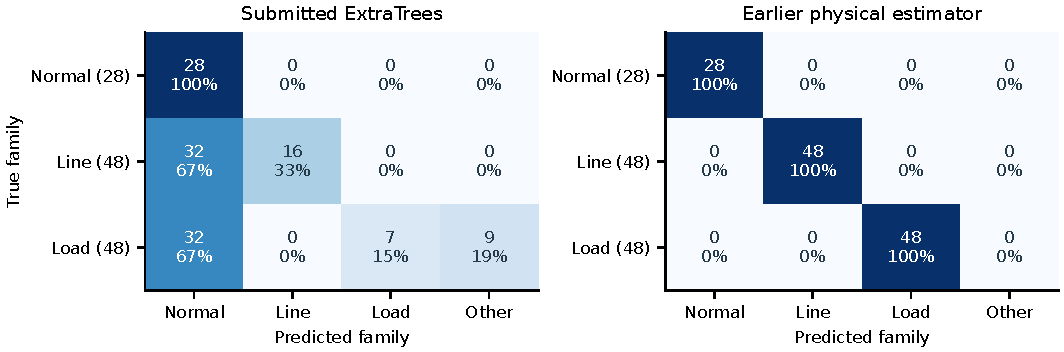
\includegraphics[width=.96\textwidth]{figures/generated/historical_transfer_confusion.pdf}
\caption{Historical development transfer on shared observation windows.
Cells show counts and row percentages. All out-of-scope predictions are
retained as ``Other''; the submitted system's nine such predictions were
the unknown-event label. This is a family matrix, not a localization
matrix. The physical comparator is an earlier estimator, not the final
continuous bank. The 96 event realizations reuse 36 physical event
trajectories; the normal windows come from six physical trajectories.}
\label{fig:historical-transfer}\end{figure*}

This comparison exposes a transfer failure of the delivered system on
the later simulator's load/line catalog. It does not show an official
hackathon-score improvement. The submitted model retains its broader
training domain and 30-s window rule, whereas the physical estimator
knows the simulator and its 12 candidate origins. These were development
cases, and the comparison permits both methods the same window endpoint.
The next study therefore uses separately trained causal ExtraTrees
comparators, successive events and a new frozen cohort. Its results must
be read as a second experiment, not as more independent repetitions of
the perfect development score.


\subsection{Following Successive Events Through Recovery}

The example in Fig.~\ref{fig:narrative-rolling} follows six physical
interventions without restarting the network. With matched R/X, all six
sources are identified before their OFF times. Under a network change
outside the bank, an extra bus-20 diagnosis precedes the real bus-31 load;
bus 31 is then diagnosed only after its physical restoration. The lower
panel shows the mechanism visible to the method: active bus-31 mass rises
late in the mismatched record. This is one development trajectory, not a
performance estimate.

\begin{figure}[t]\centering
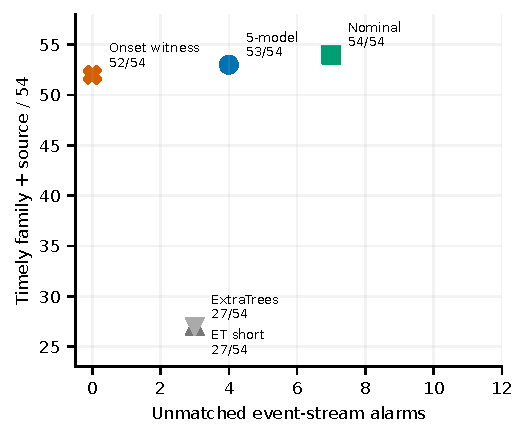
\includegraphics[width=\columnwidth]{figures/generated/narrative_tradeoff.pdf}
\caption{Development decision trade-off on 18 interventions replayed under three R/X settings. A stricter onset witness eliminates extra alarms but misses a true bus-16 load. The 54 plotted realizations share physical parents. These controls were not selected using the later sealed evaluation.}
\label{fig:narrative-tradeoff}\end{figure}

The development controls also show that deleting alarms is easy if true
events may be lost (Fig.~\ref{fig:narrative-tradeoff}). The stricter onset
witness has no extras but loses a real bus-16 intervention. The frozen
five-model procedure was therefore evaluated with its original publication
rule; no rule was revised from the sealed outcomes.

\begin{figure*}[t]\centering
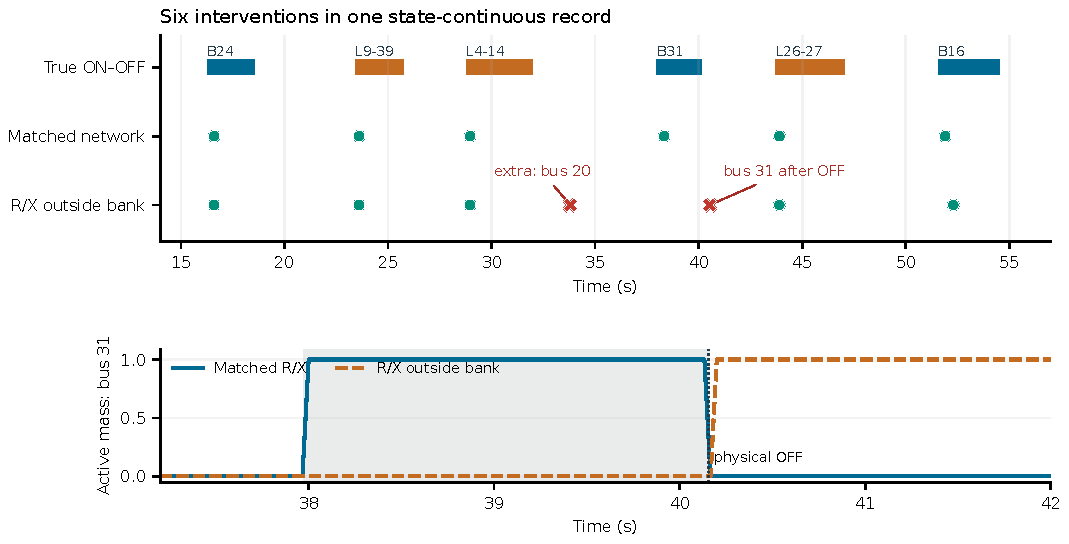
\includegraphics[width=.92\textwidth]{figures/generated/reader_episode_story.pdf}
\caption{One development sequence. Bars show reserved physical ON--OFF truth;
circles are correct diagnoses emitted before OFF; crosses mark an extra
bus-20 alarm and a bus-31 diagnosis emitted after OFF. Both lower decision
rows use the same physical bank under different R/X conditions. The lower
panel shows approximate active mass for bus 31: with R/X outside the bank,
the correct explanation becomes dominant only after restoration. Truth is
shown retrospectively and never enters inference.}
\label{fig:narrative-rolling}\end{figure*}

\subsection{Comparison With a Simpler Physical Procedure}
An earlier development control uses the same nominal physical and PMU
operators, one retained state and a short generalized likelihood-ratio
search. With a common six-report publication clock, it obtains
\SSSimpleTimely{}/\SSSimpleTotal{} timely decisions and
\SSSimpleExtras{} extras; the history mixture obtains
\SSMixTimely{}/\SSMixTotal{} with \SSMixExtras{}. This is an executed
physical comparator, separate from the later confirmatory cohort.
Different search, severity treatment and score semantics prevent it from
being a pure Bayes or memory ablation. Its equations and full table are
included in the supplement.
